\documentclass[thesis.tex]{subfiles}
\begin{document}

\chapter{Main}\label{chap:basics}

\section{Overview}
\begin{figure}[h]
	\centering
	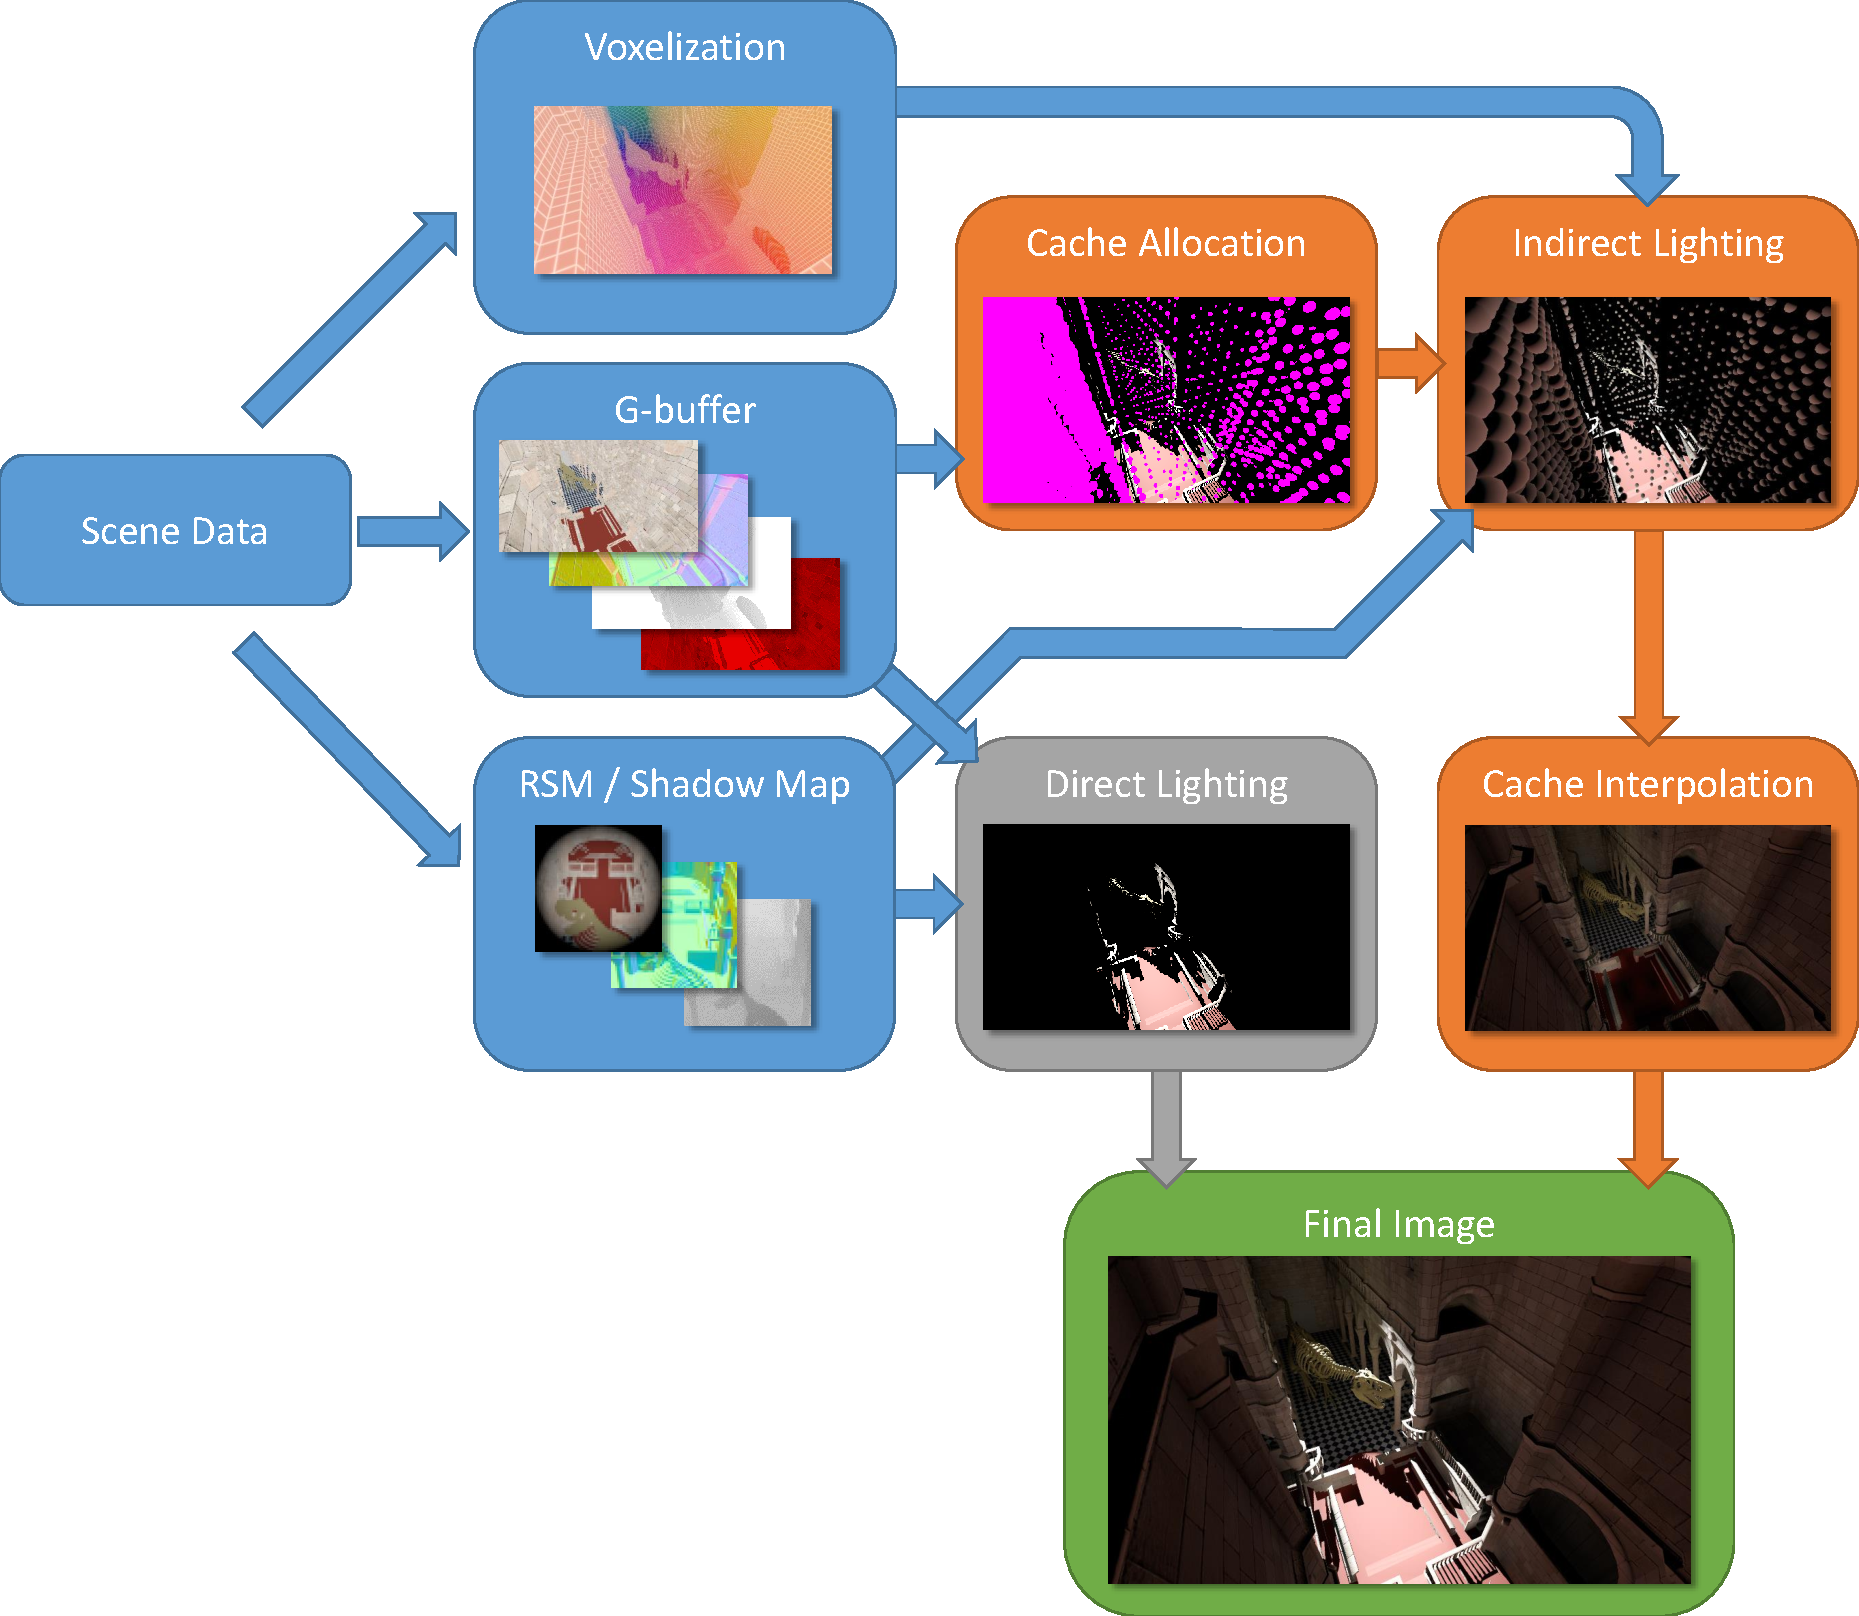
\includegraphics[width=\textwidth]{renderingpipeline.pdf}
	\caption{Overview over our basic rendering pipeline. The three steps of our technique are the orange boxes.}
	\label{fig:pipelineoverview}
\end{figure}
%
Inspired by Lensing's LightSkin approach~\cite{bib:LightskinPaper}, we want to compute indirect lighting only at specific locations and interpolate the results over multiple pixels, as opposed to techniques like reflective shadow maps or voxel cone tracing.
Like other previous works, we call these locations \emph{Light Caches}.
\\
Our technique consists of three basic steps which are executed in every frame: Cache allocation, indirect lighting and cache interpolation.
\autoref{fig:pipelineoverview} gives an overview of the pipeline steps and their dependencies.
The cache allocation pass assigns cells on a regular grid to cache memory, thus creating the caches that are about to be used in this frame.
Using a reflective shadow map, indirect lighting is then computed for all caches.
Finally each pixel interpolates an indirect lighting value using all neighboring caches within the grid.

Each of the following major sections will explain one of these stages and their interdependencies.
The last major section of this chapter will elaborate several implementation details, some of them crucial to the overall performance.\\
Many parts of our approach are based on several well-known techniques of which most have already been discussed in \autoref{chap:prevwork} and \autoref{chap:basics}.
Where necessary, details of the respective algorithms will be elaborated to address specifics implied by the overall technique.

\section{Cache Allocation}
Since the goal of this work is a fully dynamic solution that works without any pre-computations, it is necessary to place all caches at runtime, as opposed to LightSkin~\cite{bib:LightskinPaper} where caches are placed in a computational intense preprocessing step.
Instead, we use a grid based approach similar to Vardis et al. \cite{bib:radiancecachechromaticcompression}.
Before we discuss the details of our solution, several general properties and implications of such an approach are elaborated.

\subsection{General Properties of Dynamic Cache Placement} \label{sec:impl:dyncacheplace}
Compared to a pre-computation based approach, there are several intrinsic advantages which can be expected of dynamic light cache placement.
Since we try to achieve only a single bounce of indirect light, caches are only used by locations that lie in the current view frustum. % (for multiple bounces however, it might be necessary to transfer lights between caches).
It should be possible to decrease the number of caches for distant objects, thus keeping the screen-space cache density low even for high viewing ranges.
%Both properties result in a much lower memory footprint especially for large scenes.
\\
While it can be very beneficial to place caches freely, only depending on view space information may introduce several temporal artifacts if caches disappear or move. %, i.e. strong changes in indirect lighting from one frame to the next.
Additionally, it is necessary to guarantee that target pixels have easy access to a certain number of caches to be able to interpolate smoothly between them.
Note that the interpolation pass can have temporal coherence problems on its own, as the assignment of a cache to its surrounding world positions needs to be stable, no matter how densely they are sampled, i.e. how many pixels a given world space area covers.

%So far, the data requirements of each cache have not been defined yet.
Precomputed caches can naturally hold almost arbitrary data. % (as long as a given memory bound is not exceeded).
Dynamic caches on the other hand need to acquire their data every frame, which is not only costly performance-wise but may also cancel out certain types of data as it may not be accessible.
For example LightSkin~\cite{bib:LightskinPaper} needs a rather complex area metric for each cache that cannot be computed in real-time.
Naturally, such constraints also affect the following lighting and interpolation stages tremendously.

We evaluated several approaches before we came up with our final algorithm.
%If you are interested 
A summary of these attempts can be found in \autoref{chap:abandoned}.

\subsection{Cache Address Volume}
\begin{figure}[h]
	\centering
	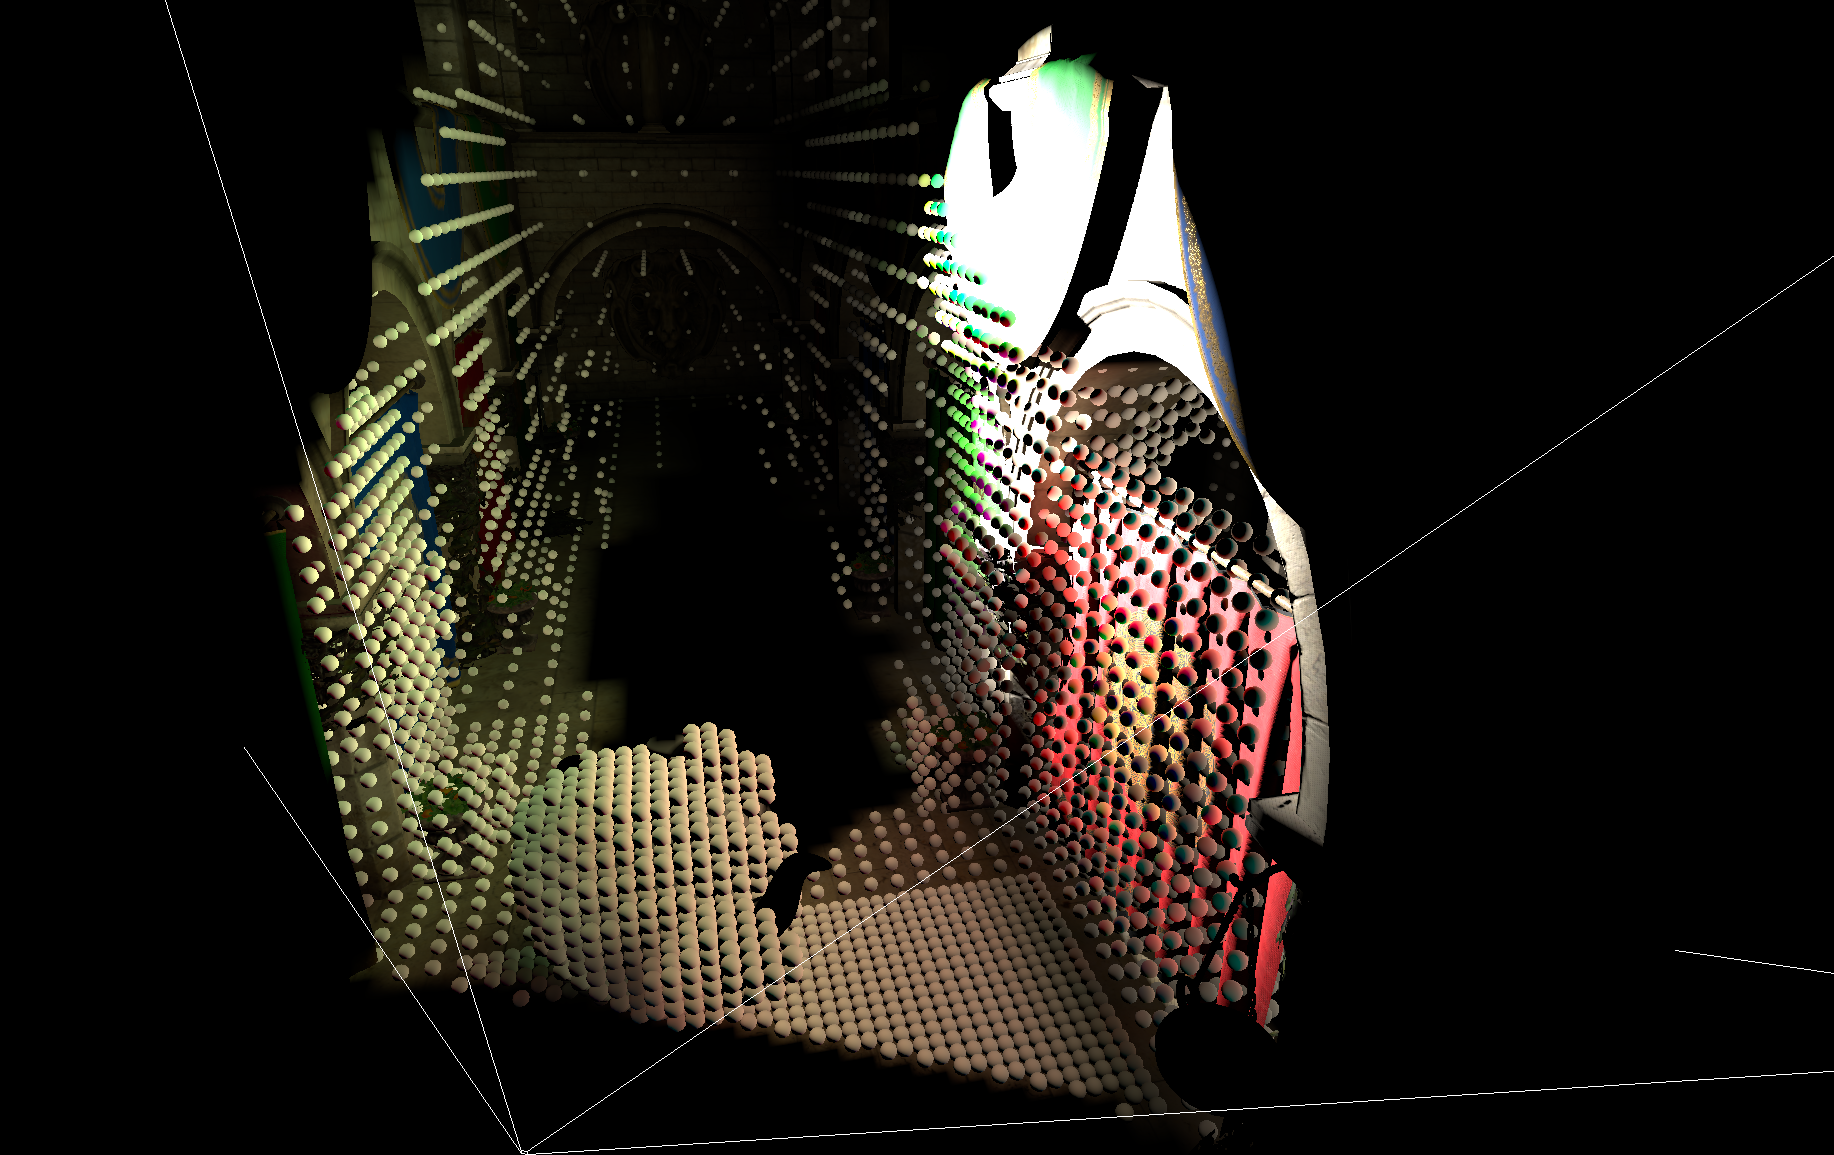
\includegraphics[width=\textwidth]{cachevis}
	\caption{Visualization of active caches for a view hinted by the white lines. Note that there is a "shadow" behind the object in the middle where no caches are active since the camera cannot see behind it.} \label{fig:cachevis}
\end{figure}
To cancel out temporal artifacts caused by moving light caches, we decided to place caches only at the nodes of a regular world space grid.
The main disadvantage of this method is that caches are not placed on surfaces and thus cannot have a specific orientation.
Since only a small fraction of all grid cells is actually needed at any time (i.e. lies near to geometry), their data is stored in a separate \emph{cache buffer} and only addresses to this buffer are saved within the grid.
Accordingly, we call this grid the \emph{cache address volume (CAV)}.
This approach reduces not only the memory consumption drastically, it makes it also much easier to perform the lighting for each cache, since those reside consecutive in a special memory block instead of being scattered within a volume as in Vardis et al. \cite{bib:radiancecachechromaticcompression}.

During the cache allocation pass the CAV is cleared and then refilled depending on the current view.
This is done by a full-screen pass, using the per-pixel world-positions from the previously rendered scene. % (which can be acquired using the depth buffer).
Each pixel allocates caches at the eight nearest CAV cells by reserving addresses and writing them into the CAV.
If however an affected cell already contains a valid cache address, it is skipped.
As pixels do not introduce any data besides the cache allocation itself no additional writes are needed.
Since neighboring pixels often access the same grid cells, there is room for some effective optimizations using shared memory which are explained in \autoref{sec:impl:cachealloc}.
\autoref{fig:cachevis} shows a resulting cache distribution already with CAV cascading which is explained in the next section.

\subsubsection{Cascading} \label{sec:impl:cavcascading}
\begin{figure}[h]
	\centering
	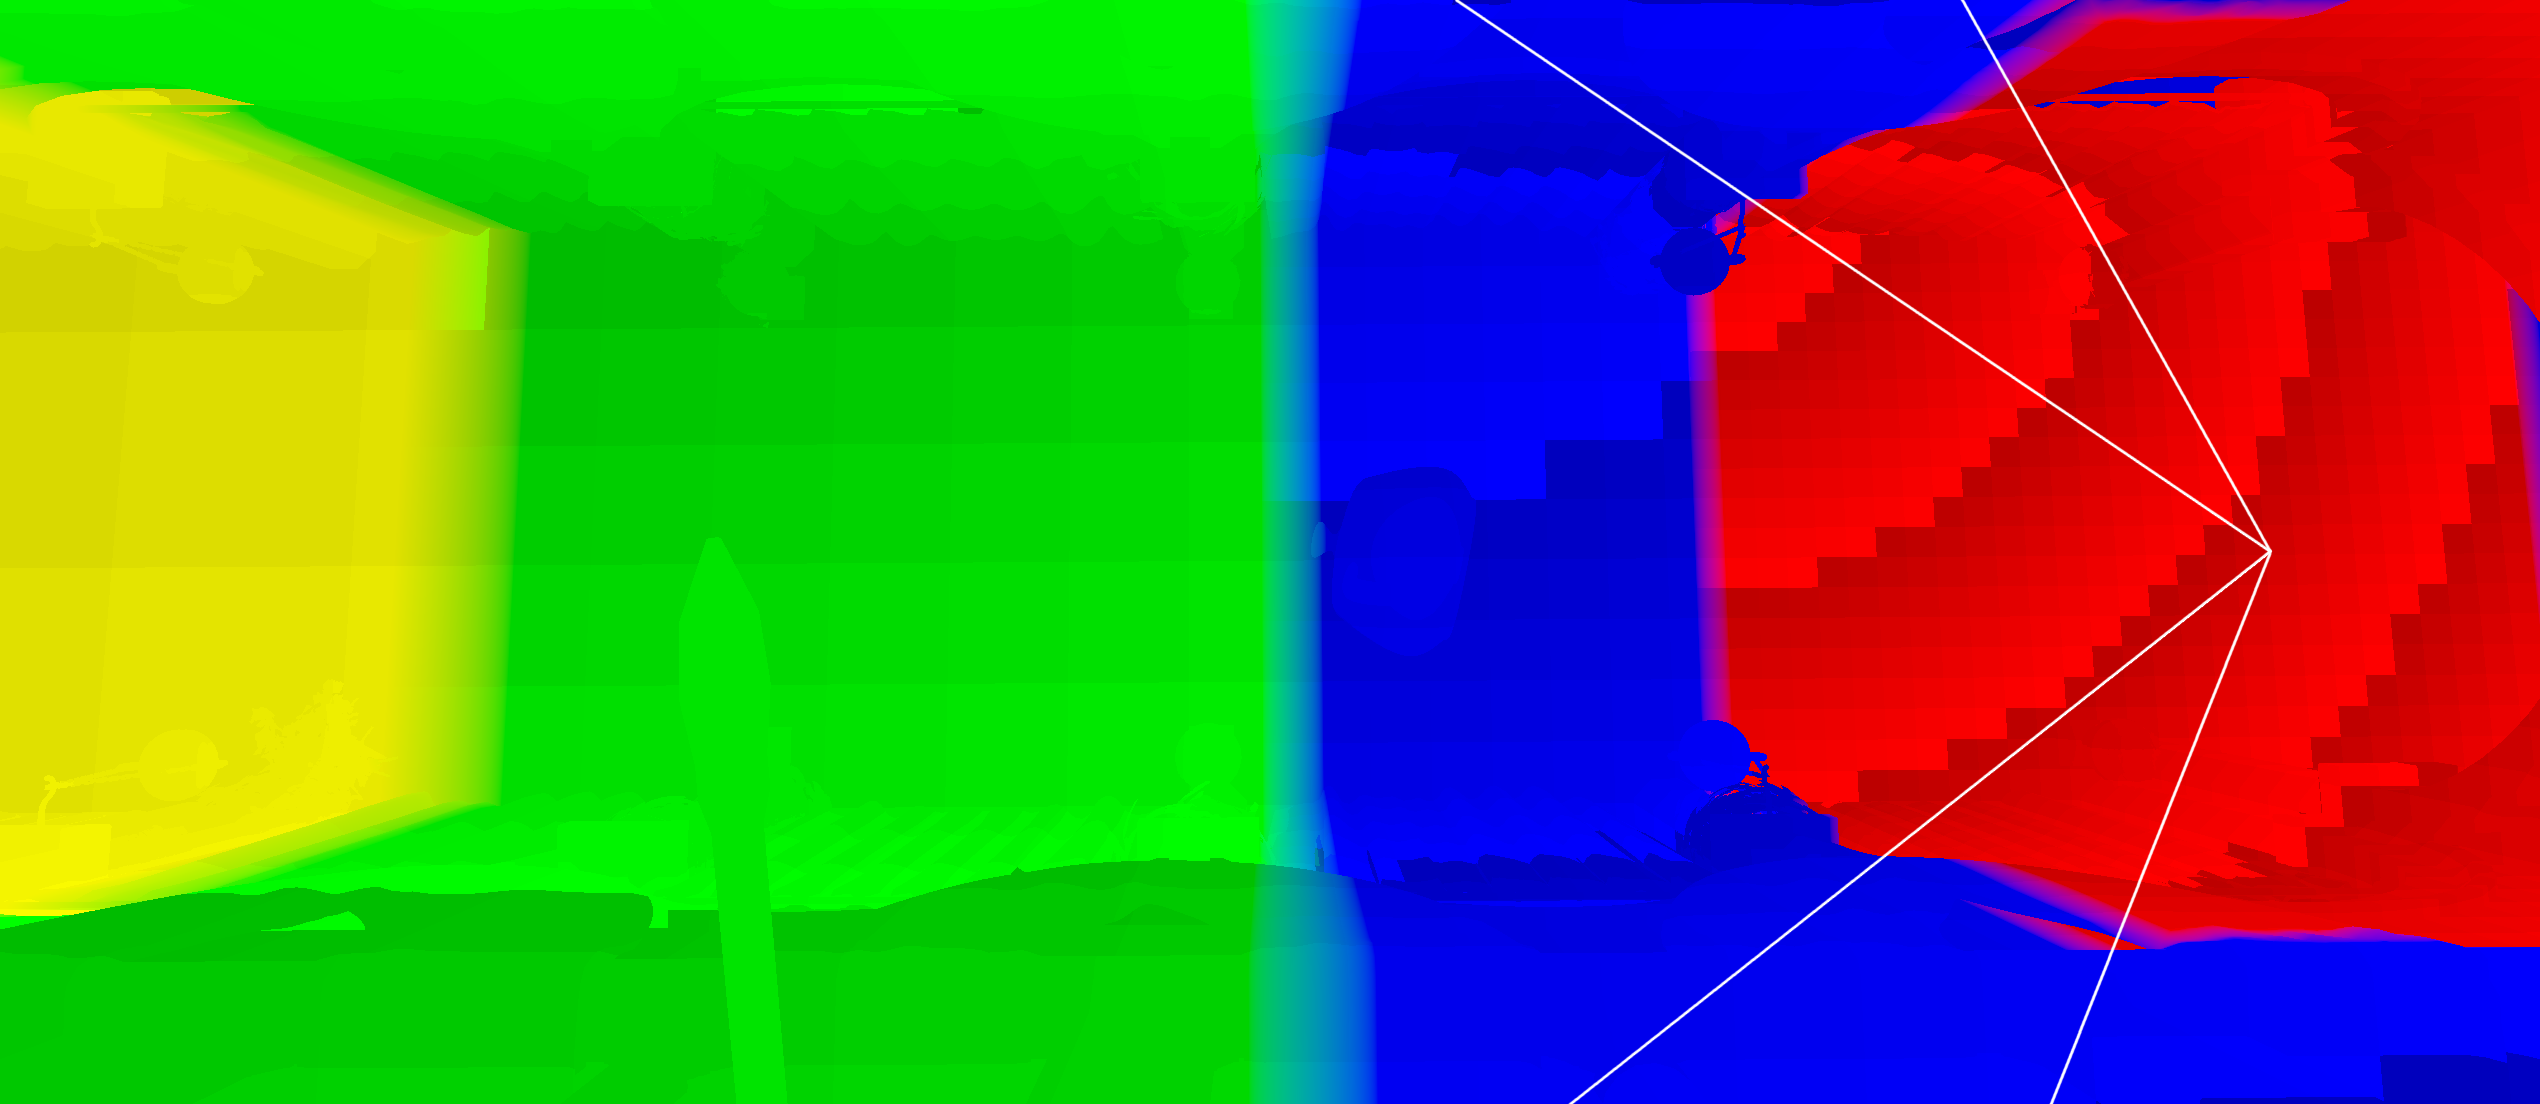
\includegraphics[width=\textwidth]{cascades}
	\caption{Visualization of CAV cascades. Again, the white lines to the right show the active view frustum.
	Areas with the same brightness within a cascade (single colored area) indicate the local cache size.
	%The brightness differences within a cascade (single colored area) hint the cache size.
	} \label{fig:cavcascades}
\end{figure}
Similar to Cascaded Light Propagation Volumes \cite{bib:lpt} a set of nested CAV cascades is centered on the camera.
\autoref{fig:cavcascades} visualizes the cascading system.
This introduces a distance-dependent level of detail and keeps the number of caches at a reasonable level, even for large scenes.
The cascade positions are snapped to multiples of their grid size to ensure consistent lighting results. %\todo{elaborate the snapping-whys further?}
For simplicity, all CAV cascades are cubic and have the same resolution, while their grid size is doubled for each consecutive cascade.

Caches are only allocated in the smallest CAV cascade which encloses a given pixel world-position.
To be able to allocate all eight nearest CAV cells in a single cascade, special "decision boundaries" which are smaller than the actual cascade are used for cascade selection.
As the snapped movement introduce temporal incoherency, we move the decision boundaries smoothly with the camera and shrink them further by another grid cell size to ensure that they are fully enclosed by their respective cascades.
\\
Additionally, there are transition areas between two successive cascades.
Within these areas, caches are allocated in both cascades to be able to avoid hard edges during the interpolation stage later on.
The size of the transition areas can be chosen freely.
For our demos we use transition areas as wide as the cell size of the next bigger cascade. %as wide as twice the cell size of the smaller involved cascade.
This delivers sufficiently smooth transitions for reasonable performance costs in our scenes.

Contrary to Light Propagation Volumes, the cascades are not offset depending on the camera direction.
Instead they are strictly centered on the camera position as this helps to keep the level of detail stable for view rotations.\\
While this means that a very large portion of each cascade is never used at all, the costs are still rather low since there are no computations involved for empty cells.
Also, the memory footprint is still rather small: %nevertheless
A highly detailed setup consists of four cascades, each with a resolution of $64^3$.
With a four byte address in each cell, this makes only four megabytes for all CAV cascades together.

\section{Indirect Lighting}
The indirect lighting of the caches relies on reflective shadow maps (see \autoref{sec:prev:rsm}).
In principle each cache iterates over the entire RSM to retrieve the encoded lighting information.
This section explains how this information is processed and how the results are saved for later interpolation.

\subsection{RSM Preparation} \label{sec:impl:rsmprep}
We render the RSM in a relatively high resolution (usually $1024^2$) and sample it down for the upcoming indirect lighting steps (usually from $16^2$ up to $128^2$).
%For the down-sampling
In the process depth values and normals are averaged, while flux values are summed to preserve energy.
For geometry with many depth discontinuities, this improves the temporal coherence under movement of both objects or lights.
This approach may result in incorrect virtual lights, floating in midair with normals vectors that are not present in the original RSM samples.
However, we have not encountered any visible artifacts resulting from this filtering technique in our tests.
\\
The direct lighting process uses the original depth from the RSM as shadow map.
In the following sections the term RSM denotes the already down-sampled texture set.

\subsection{Diffuse Lighting} \label{sec:impl:diffuse}
We separate diffuse and specular lighting, making the later an optional feature that may be deactivated to save resources if necessary.
Diffuse lighting is comparatively easy to represent and compute since it is (for a given position and reflectivity) a low frequency function over a surface normal, independent of the current view direction.

%The rendering equation for pure diffuse surfaces is defined as follows (compare \autoref{sec:preq:brdf} and \autoref{sec:preq:renderingeq}):
%\begin{equation}
%L_d (\mathrm{x}) = \frac{\rho_d}{\pi}\int\limits_{2\pi\,sr} L_i(x,\omega_i) \cdot \cos\theta_i \,\mathrm{d}\omega_i
%\end{equation}

Recall the definition for lighting with $M$ virtual lights (see \autoref{sec:prev:manylights}):
\begin{equation}
L(\mathrm{x}, \omega_o) = \sum\limits_{i=1}^{M} f_r(\mathrm{x}, \overrightarrow{\mathrm{x}\mathrm{x}_i}, \omega_o) \cdot G(\mathrm{x}, \mathrm{x}_i) \cdot \hat{V}(\mathrm{x}, \mathrm{x}_i) \cdot I_i(\overrightarrow{\mathrm{x}_i\mathrm{x}})
\end{equation}
We use the geometry term $G$ for disc shaped area lights by Lensing et al. \cite{bib:LightskinPaper} as mentioned in \autoref{sec:fig:rsmbias}.
The visibility function $\hat{V}$ is ignored for now, it is handled later on in \autoref{sec:main:shadowing}.
Since we are only interested in diffuse lighting, the BRDF $f_r$ and the VAL's intensity curves $I_i$ are rather simple:
\begin{align}
f_r(\mathrm{x}, \overrightarrow{\mathrm{x}\mathrm{x}_i}, \omega_o) =& \frac{\rho_d}{\pi}\\
I_i(\overrightarrow{\mathrm{x}_i\mathrm{x}}) =& \frac{\rho_i}{\pi} \phi_i
\end{align}
The final expression for diffuse indirect lighting is accordingly defined as follows:
\begin{equation} \label{eq:rsmdiffuse}
L_d (\mathrm{x}) = \frac{\rho_d}{\pi} \sum\limits_{i=1}^{M} 
(\hat{\mathbf{n}} \cdot \overrightarrow{\mathrm{x}\mathrm{x}_i} )^+ \cdot
\underbrace{\frac{(\hat{\mathbf{n}}_i\cdot \overrightarrow{\mathrm{x}_i\mathrm{x}})^+}{||\mathrm{x} - \mathrm{x}_i||^2 + A_i} \cdot  \frac{\rho_i}{\pi} \phi_i}_{L_i}
\end{equation}
The diffuse reflectivity $\rho_d$ at the point $\mathrm{x}$ is factored out - it can be applied easily during the cache interpolation stage.
Like the position of a virtual area light, its area $A_i$ can be computed from the depth values saved in the RSM.
Lensing et al. \cite{bib:LightskinPaper} use the following surface independent estimation for a virtual light $i$ at the distance $z_i$ from the source light (which is stored in the RSM):
\begin{equation}
A_i = z_i^2 \cdot \frac{A_{near}}{z_{near}^2 M}
\end{equation}
We assume a quadratic RSM with a total of $M$ pixels with a near plane area of $A_{near}$ at a distance of $z_{near}$.

Our cache grid effectively quantifies the range of positions $\mathrm{x}$ in which the sum over all virtual lights is evaluated.
Since caches are not placed on surfaces, the normal vector $\hat{\mathbf{n}}$ is not known in advance.
Therefore, we save the incoming radiance $L_i$ as a function over the sphere in each cache to integrate it later on with a cosine lobe, i.e. weighting every direction with the dot product between the surface normal and the direction.
As in many previous works, we choose a spherical harmonics representation with either two or three bands to approximate this function.
The SH representation allow iterative computation and easy evaluation.

To perform the diffuse cache lighting, the SH coefficients for all virtual lights are accumulated and saved into the cache buffer for later evaluation.
%Depending on the demanded accuracy we use the first two or three SH bands.
The impact on performance and quality of varying number of SH bands will be discussed in \autoref{sec:eva:shperf} and \autoref{sec:eva:shquality}.

\subsection{Specular Lighting} \label{sec:impl:specenvmap}
As mentioned in \autoref{sec:preq:brdf} we make use of a normalized version of the Blinn-Phong BRDF.
Using virtual point lights from the reflective shadow map, the specular part of the visible radiance is defined as following:
\begin{equation}
L_s (\mathrm{x}) = \rho_s \cdot \frac{\gamma + 8}{8\pi} \cdot \sum\limits_{i=1}^{M}
(\hat{\mathbf{n}}\cdot \overrightarrow{\mathrm{x}\mathrm{x}_i})^+ \cdot L_i \cdot ((\hat{\mathbf{n}} \cdot \hat{\mathbf{h}}_i)^+)^\gamma
\end{equation}
Where $\hat{\mathbf{h}}_i$ is the half vector to the $i$th light and $\gamma$ the specular exponent.
The incoming radiance $L_i$ from a light was defined in \autoref{eq:rsmdiffuse}.
\\
For moderately high $\gamma$ the outgoing specular radiance is, contrary to outgoing diffuse radiance, a high frequency function over $\hat{\mathbf{n}}$.
Using the same representation as in the previous section on diffuse lighting would require to evaluate much more SH bands (e.g. as in radiance caching \cite{bib:radiancecaching}) which are difficult to compute and prone to ringing artifacts.
%Instead, an image based approach is used

\begin{figure}[h!]
\centering
\subcaptionbox{Cache visualization displaying indirect specular reflections.}{
	\begin{subfigure}[b]{1.0\textwidth}
		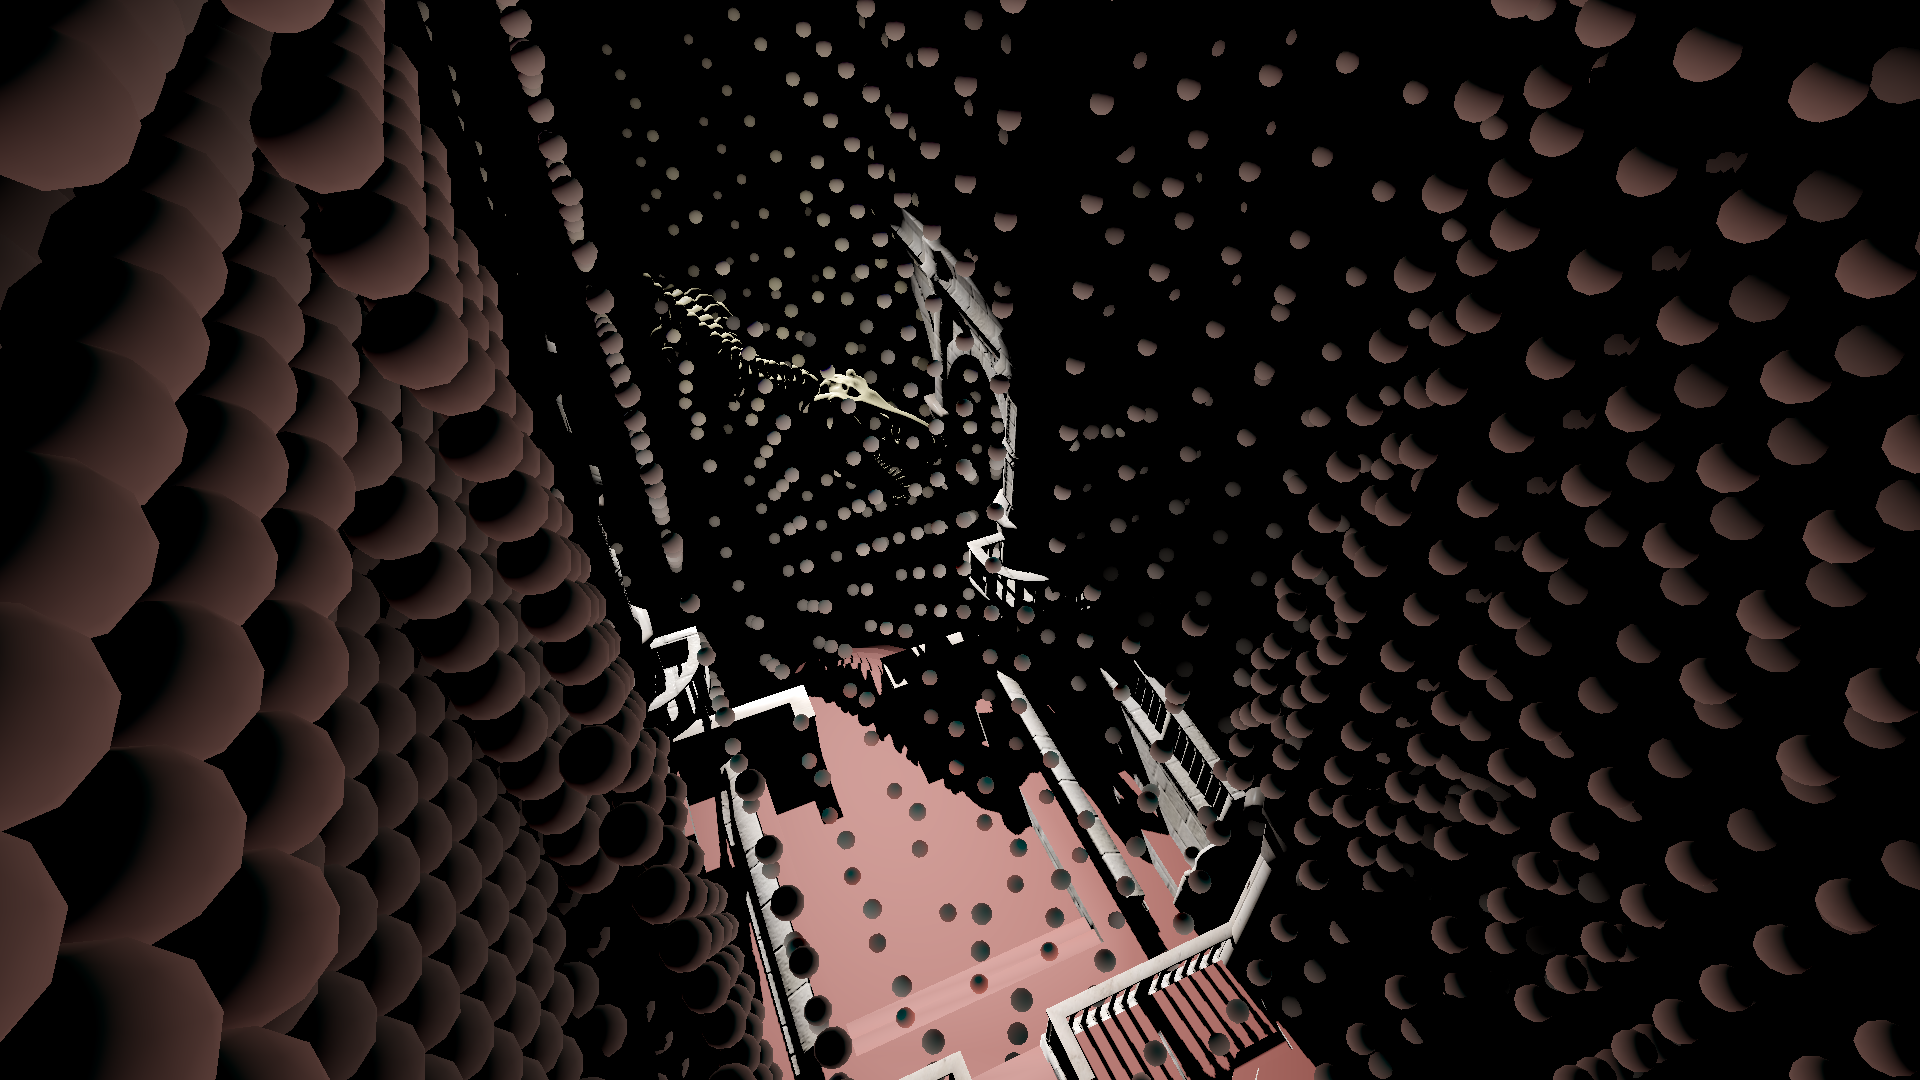
\includegraphics[width=\textwidth]{specularenvmap/caches}
   	\end{subfigure}
}
\\
\subcaptionbox{Cut-out of the texture atlas.}{
	\begin{subfigure}[b]{0.7\textwidth}
		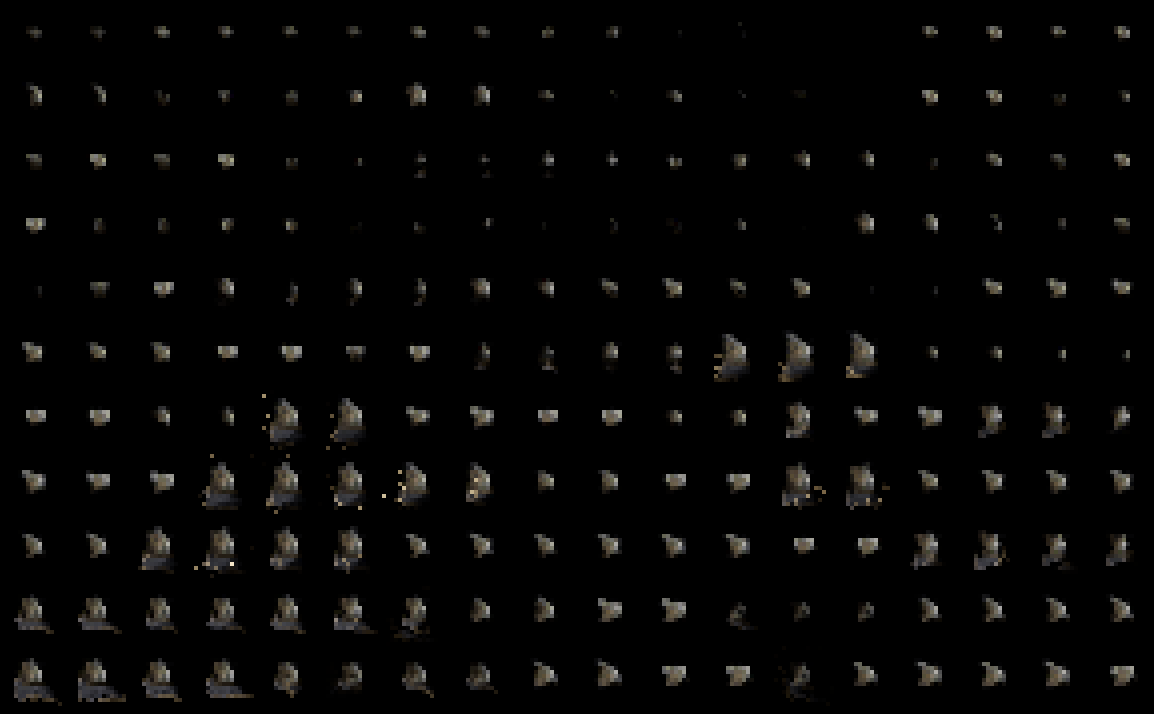
\includegraphics[width=\textwidth]{specularenvmap/atlas}
   	\end{subfigure}
}
\caption{Visualizations of the specular environment map, using $16^2$ pixels per cache.}
\label{fig:specularenvmap}
\end{figure}
If it is assumed that a cache lies directly on a \emph{visible} surface, then the space of possible normal vectors is limited to the hemisphere pointing towards the viewer.
We need to record outgoing radiance (again postponing the factors outside of the sum) for every direction on  the hemisphere for each possible $\gamma$.
As the outgoing radiance for lower exponents can be estimated by integrating results for higher $\gamma$ values, only an upper bound $\gamma_{max}$ is handled for now.
For very large $\gamma_{max}$, the $((\hat{\mathbf{n}} \cdot \hat{\mathbf{h}}_i)^+)^{\gamma_{max}}$ term is only bigger than zero if $\hat{\mathbf{n}} \cong \hat{\mathbf{h}}_i$.
This means that in the limit each given virtual point light contributes only to a single hemisphere direction.
\\
We discretize the hemisphere into a limited number of directions.
Using the large $\gamma_{max}$ assumption, we apply light only to the nearest discrete direction.
Similar to the work of McGuire et al. \cite{bib:envmipmap} on plausible Blinn-Phong cubemaps, we require that the solid angle of the given Blinn-Phong lobe does not exceed the angle between two data points.
This allows to compute a plausible value for $\gamma_{max}$, given a number of $D$ uniformly distributed directions.
\begin{align}
\int\limits_{2\pi sr} (\cos\theta)^{\gamma_{max}}  \,\mathrm{d}\omega = \frac{2\pi}{D}\\
\gamma_{max} = D-1
\end{align}
%
To be able to efficiently address values per direction on a texture, the hemisphere is projected onto a square.
First, all directions are expressed in the local view space, which is a transformation that maps the direction to the camera to $(0,0,1)$ .
For the projection itself it is important that it introduces as little distortion as possible since otherwise the directions are no longer distributed equally.
For this purpose we use uniform concentric maps by Shirly and Chiu \cite{bib:concentricmaps}.
We call the resulting maps \emph{specular environment maps} and store them in a large texture atlas.
The atlas can easily be addressed by the cache address which was already used for the cache buffer.
Depending on the quality setting, each cache uses typically a resolution between 8x8 and 32x32 pixels on this atlas.
After all caches are lit, mipmaps of the Specular Environment Map atlas are created.
Similar to classical reflection maps \cite[p.~308]{bib:RealtimeRenderingBook} they will later be used to estimate the specular lighting for Blinn-Phong exponents bellow $\gamma_{max}$.
\\
\autoref{fig:specularenvmap} shows visualizations of the specular environment map.
We found that the method has some weak points that will be later discussed in \autoref{sec:eva:specperf} and \autoref{sec:eva:specquality}.


\subsection{Indirect Shadows} \label{sec:main:shadowing}
So far, indirect visibility was ignored.
In most cases however, approximate shadows are extremely important to the overall image quality, as seen in \autoref{fig:indirectshadowonoff}.
This chapter presents a voxel cone tracing based approach with several adjustments and new simplifications that fit well in our framework.
\begin{figure}[h!]
\centering
\begin{subfigure}[b]{\textwidth}
	\includegraphics[width=\textwidth]{indirectshadow/off}
\end{subfigure}

\vspace{8pt}
\begin{subfigure}[b]{\textwidth}
	\includegraphics[width=\textwidth]{indirectshadow/on}
\end{subfigure}
\caption{A scene using our indirect diffuse lighting without (top) and with (bottom) indirect shadows.}
\label{fig:indirectshadowonoff}
\end{figure}

\subsubsection{Shadow Cone Tracing}\label{sec:impl:voxelization}
To estimate shadowing effectively, we trace cones from the caches to virtual lights within a binary voxelization of the scene.
The general approach is very similar to the cone tracing step in Layered Reflective Shadow Maps from Sugihara et al. \cite{bib:layeredrsm}. % (as mentioned in \autoref{sec:prev:voxelcone}).
By averaging the occlusion percentage, mipmaps are created from the initial binary data (where the occlusion percentage is either zero or one).

Higher mip-levels tend to have too low occlusion values since we voxelize only surfaces.
Instead, a solid voxelization would be required.
However, such solid voxelizations are not only computational more intense, they also require a clear cut definition of the outer and inner volume which is not given by most triangles meshes.

\subsubsection{Cone Trace LOD}
Contrary to both Sugihara's layered reflective shadow maps and Crassin's voxel cone tracing we do not use the cone tracing to look up a pre-filtered lighting value.
Instead, the tracing is only used to determine if a given virtual light is visible from the position of a cache.
We found, that tracing a cone to every virtual light is, depending on the RSM resolution, usually too expensive.
However, most virtual lights lie very close in space and do not need to be tested separately.
To test multiple VALs at once we need an estimate of their spatial distribution.
%To be able to exploit this property and reduce the number of needed cones, we pre-filter the depth map of the reflective shadow map.
Inspired by Variance Shadow Maps from Donnelly and Lauritzen \cite{bib:vsm}, we save not only depth but also squared depth in the reflective shadow map and pre-filter the combined depth texture by creating mipmaps.
As in Variance Shadow Maps, the squared depth will be used to retrieve the variance of the depth value.
We introduce the \emph{Indirect Shadow LOD} as a global constant parameter that determines for which mip-level cones are traced to check the visibility of the underlying group of virtual lights (0: for each VAL, 1: every four, 2: every 16, ...).
All other lighting computations will still work on the lowest mip-level but use the previously computed shadowing value which stays the same across multiple lights.\\

\begin{figure}[h]
	\centering
	\includepdftex{shadowconetracelod}
	\caption{Shadow cone tracing from a cache (grey circle left) to a group of virtual lights (black crosses). The opening angle of a shadow cone depends on the sphere around the virtual lights which is the maximum of the projected sample width (red) and the depth variance (blue).} \label{fig:shadowcone}
\end{figure}
The pre-filtered depth texture is now used to estimate the angle of a cone that encloses a group of virtual lights.
To do so, a sphere around the concerning virtual lights needs to be estimated.
\autoref{fig:shadowcone} illustrates the algorithm.
The center of the sphere (green cross in \autoref{fig:shadowcone}) is determined directly by the shadow sample position and its depth which is the average of all underlying virtual lights.
%Both are implicitly separate averages over all underlying virtual lights.
For the radius the maximum of two separate estimations $r_{e1}$ and $r_{e2}$ is used.
\\
The first estimate $r_{e1}$ is based on an distribution estimate of light depth values:
If it is assumed that the depth values are normally distributed, approximately $95\%$ of all values lie within the range of two times their standard deviation (blue line in \autoref{fig:shadowcone}).
\begin{align}
E(d) =& \frac{1}{N} \sum\limits_{i=1}^{N} d_i\\
E(d^2) =& \frac{1}{N} \sum\limits_{i=1}^{N} d_i^2\\
\sigma^2 =& E(d^2) - E(d)\\
r_{e1} =& \sqrt{E(d^2) - E(d)}
\end{align}
The average depth $E(d)$ and averaged squared depth $E(d^2)$ of the virtual lights are available through the pre-filtered depth texture.
\\
While the first estimate works well if the virtual lights have very different distances to their origin-light, it underestimates if they are parallel to the near plane of the origin-light.
Thus, the second estimate (depicted red in \autoref{fig:shadowcone}) is the size of the sample area, projected to the center of the sphere.
The sample area is determined by the relative sample size, given by the width $w_{near}$ and depth $z_{near}$ of the near clip plane, the RSM resolution $R$ and the chosen Indirect Shadow LOD $l$.
\begin{equation}
r_{e2} = E(d) \cdot \frac{w_{near}}{z_{near} \cdot R \cdot 2^{-l} }
\end{equation}

\subsubsection{Cone Trace Sampling Steps}
\begin{figure}[h]
	\centering
	\includepdftex{conetracestep}
	\caption{Sampling a shadow cone from a cache to a light(-group). The first two enclosing circles do not touch each other because the sample distance would then below the minimum.} \label{fig:shadowconestep}
\end{figure}
The ray from cache to the sphere is sampled in increasing steps.
%Starting with a step size of one voxel width, the steps are doubled with each additional sample.
For each sample, we need to determine the mip-level in the voxel-volume of which a single voxel is approximately as large as the cone segment that is represented by the sample.
This is estimated by the radius $r_s$ of the inner circle of the current sample, as depicted in \autoref{fig:shadowconestep}.
It can be computed by easy trigonometry:
\begin{equation}
r_s = d_s \cdot \sin \alpha = d_s \cdot \frac{max(r_{e1}, r_{e2})}{||\mathrm{c} - \mathrm{l}||}
\end{equation}
$d_s$ is the distance of the given sample to the cache. $\mathrm{c}$ and $\mathrm{l}$ are the positions of the cache and light.
The cone angle $\alpha$ does not need to be evaluated directly. % at any time.
If all values are given in voxel volume coordinates, the sampled mip-level is simply $log_2(r_s)$.\\
The distance $d_s$ of the next sample is chosen so that two inner circles touch each other:
\begin{align}
d_{s'} =& d_s + r_s + r_{s'} = d_s + r_s + d_{s'} \cdot \sin \alpha\\
d_{s'} =& \frac{d_s + r_s}{1-\sin\alpha} = \frac{d_s + r_s}{1-\frac{r_s}{d_s}} 
\end{align}
To avoid needless oversampling for thin cones, step sizes smaller than one voxel are no allowed (as illustrated by the first two samples in \autoref{fig:shadowconestep}).

Using a trilinear texture filter, the opacity values $\alpha_s$ from the voxel volume are interpolated within and across mip-levels.
The total visibility $V$ is accumulated front to back:
\begin{equation}
V = 1 - \sum\limits_{s=1}\alpha_s \prod\limits_{j=0}^{s-1}(1-\alpha_j)
\end{equation}
The sampling stops if either the light group position $\mathrm{l}$ is reached or the visibility approaches zero.

\section{Cache Interpolation}
After all caches have been populated with lighting data, their information needs to be interpolated across the screen.
As in the cache allocation pass, each pixel uses its world position to retrieve the buffer locations of its eight nearest caches in one or two cascades (for transitions).
 
For the diffuse lighting, the irradiance is evaluated with the per-pixel normal in each cache.
To do so, the radiance SH needs to be integrated over the cosine weighted hemisphere.
This requires to express the cosine lobe in SH representation and perform the dot product with the irradiance SH coefficients.
Since this weight function is radially symmetric to the normal vector, rotated Zonal Harmonic coefficients can be used to derive the expression easily.
First, Zonal Harmonic coefficients $z_l$ are computed for a fixed normal direction, pointing to $(0,0,1)$.
\begin{align}
z_l =&\int\limits_{2 \pi sr} L_i \cdot (\omega \cdot (0,0,1))^+ \cdot y^0_l(\omega) \,\mathrm{d}\omega\\
=&\int\limits_{2 \pi sr} L_i \cdot \cos\theta \cdot y^0_l(\omega) \,\mathrm{d}\omega
\end{align}
Note that by integrating only over the upper hemisphere, the cosine does not need to be explicitly clamped.
Due to the rotational invariance of Spherical Harmonics, the resulting Zonal Harmonics coefficients can be rotated to the normal direction (see \autoref{sec:preq:zonalharmonics}) without data loss.
The resulting expressions for the first three SH bands can be found in \autoref{chap:shcosinelobe}.

The result is trilinearly interpolated depending on the relative position of the pixel to its eight nearest caches.
To retrieve the final visible radiance, the interpolated radiance value is then multiplied with the diffuse reflectance divided by $\pi$ (see \autoref{sec:preq:brdf}).

For the specular lighting we need to determine the relative coordinate and, depending on the Blinn-Phong exponent, at which mip-level the specular environment map of each cache should be sampled.
Identical to the computation of the specular environment map, finding the coordinate involves the projection of the normal vector using the local view space (see \autoref{sec:impl:specenvmap}).
Since the direction to the camera varies only little from cache to cache, we use the local view space at the pixel-position for all caches.
This introduces a slight inaccuracy but circumvents the possibility that a per-pixel normal vector might lie outside of a cache's local view hemisphere.\\
The mip-level is computed similarly to $\gamma_{max}$ as before, only that this time the mip-level $m$ is searched for.
\begin{align}
\int\limits_{2\pi\,sr} (\cos\theta)^{\gamma}  \,\mathrm{d}\omega = \frac{2\pi}{R \cdot 2^{-m}}\\
\frac{2\pi}{\gamma + 1} = \frac{2\pi}{R \cdot 2^{-m}}\\
m = \log_2 \Big(\frac{2 \cdot R^2}{\gamma + 1} \Big) \cdot \frac{1}{2}
\end{align}
Where $R$ is the resolution of a single specular environment map.
As before with the diffuse lighting, the results of all caches are trilinearly interpolated and multiplied with the specular reflectivity of the corresponding pixel.

Pixels in transition areas (see \autoref{sec:impl:cavcascading}) compute two radiance values, one for both CAV cascade.
The results are then interpolated linearly.


\section{Implementation Details}
In this section we provide several details of our implementation which is freely available on GitHub (\url{https://github.com/Wumpf/DynamicRadianceVolume}).
The implementation runs entirely on the GPU and makes use of several OpenGL 4.5 features.
%As we have already pointed out in \autoref{sec:preq:gpu} we make use of modern OpenGL 4.5 features like compute shaders.

\subsection{Material Setup and Direct Lighting}
\begin{figure}[h!]
\centering
\subcaptionbox{Color}{
\begin{subfigure}[b]{0.22\textwidth}
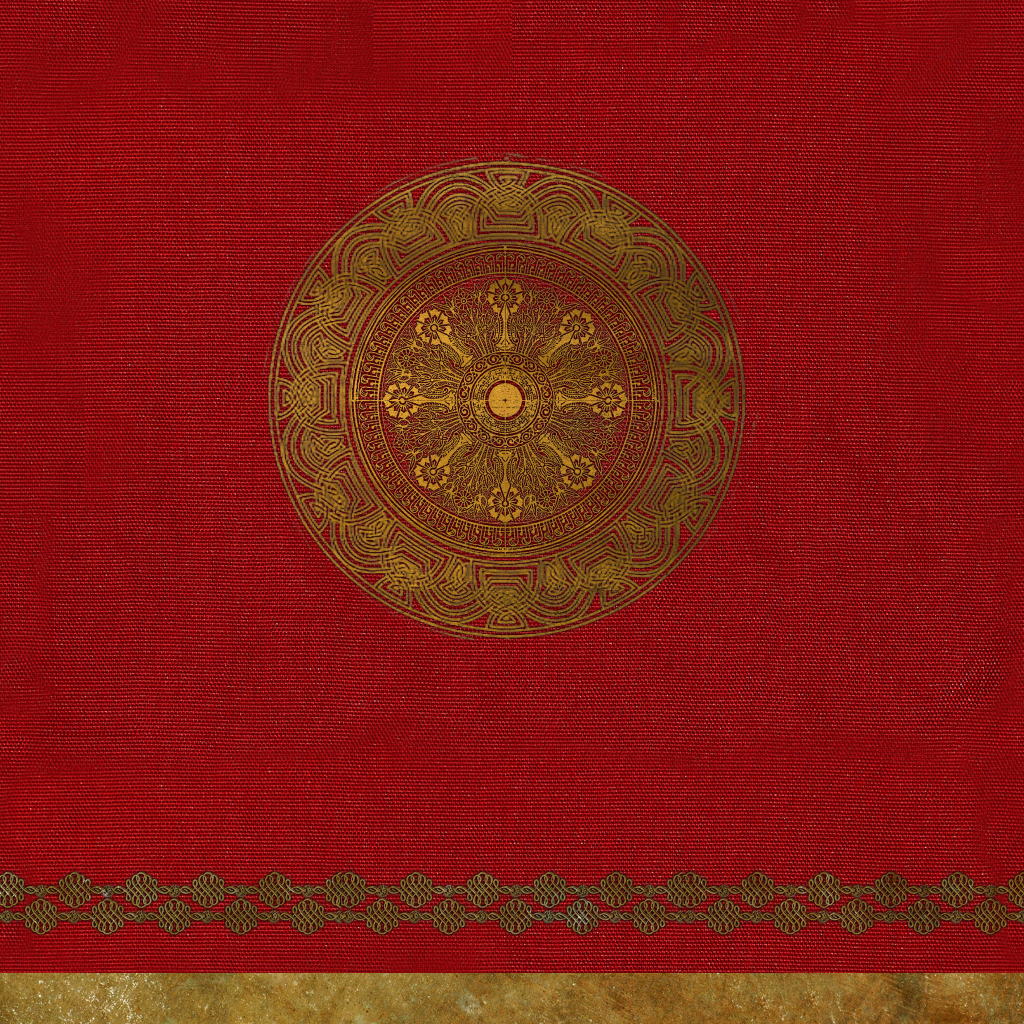
\includegraphics[width=\textwidth]{texture_sample/curtain_color}
\end{subfigure} }
\subcaptionbox{Normalmap}{
\begin{subfigure}[b]{0.22\textwidth}
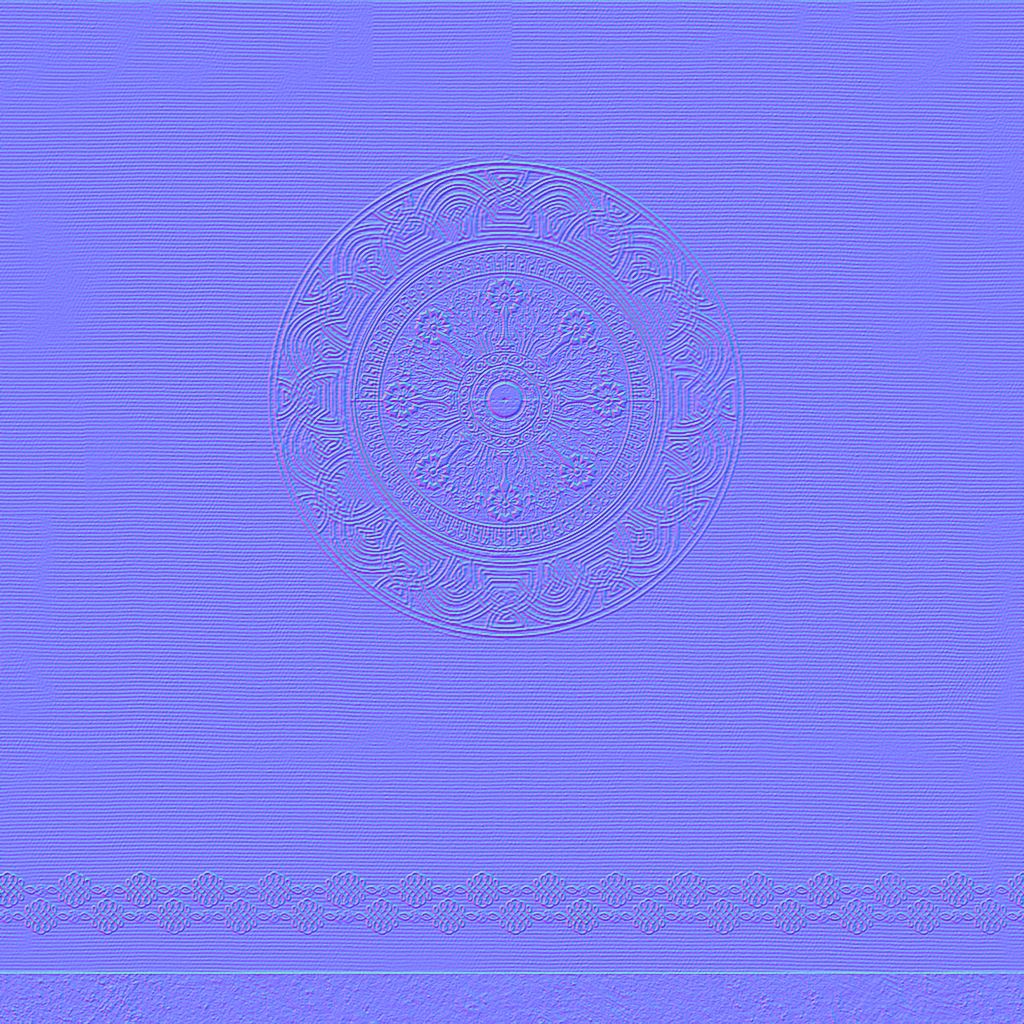
\includegraphics[width=\textwidth]{texture_sample/curtain_normal}
\end{subfigure} }
\subcaptionbox{Roughness}{
\begin{subfigure}[b]{0.22\textwidth}
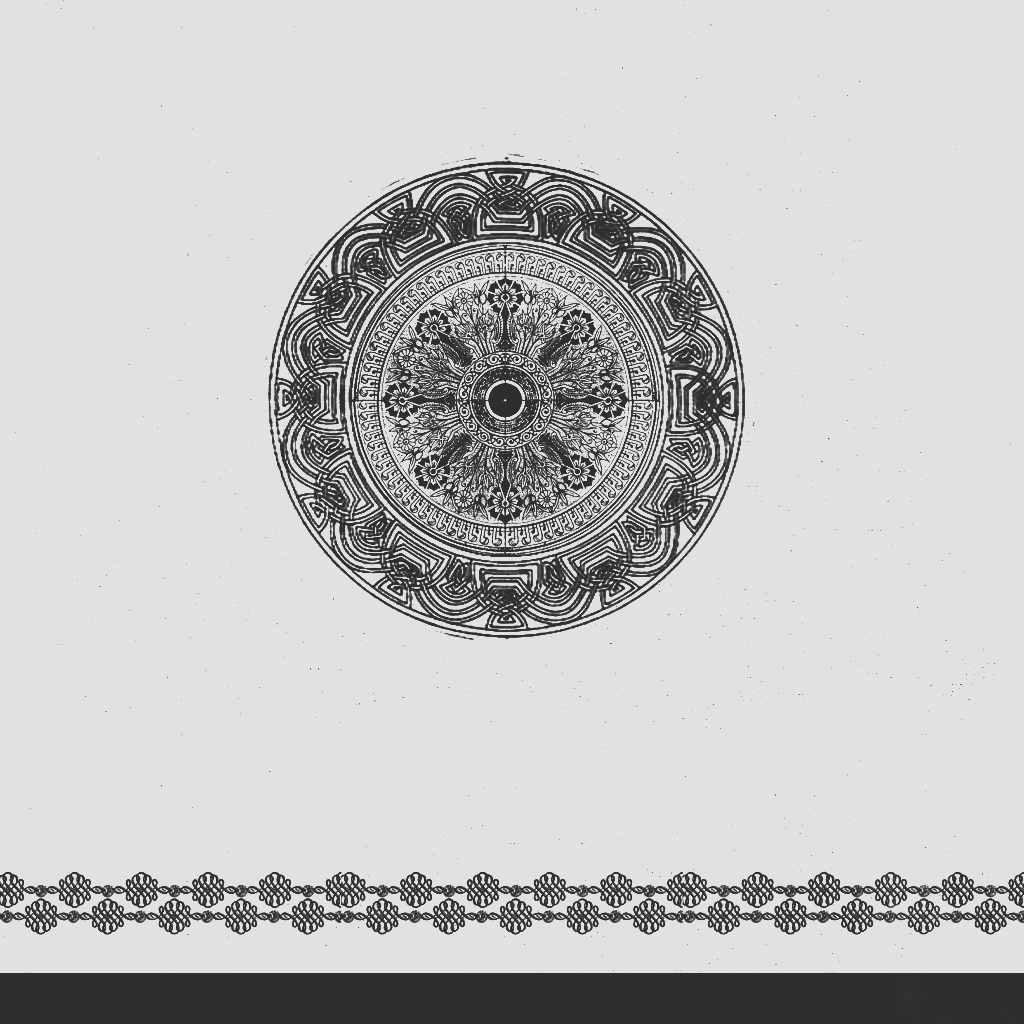
\includegraphics[width=\textwidth]{texture_sample/curtain_roughness}
\end{subfigure} }
\subcaptionbox{Metallic}{
\begin{subfigure}[b]{0.22\textwidth}
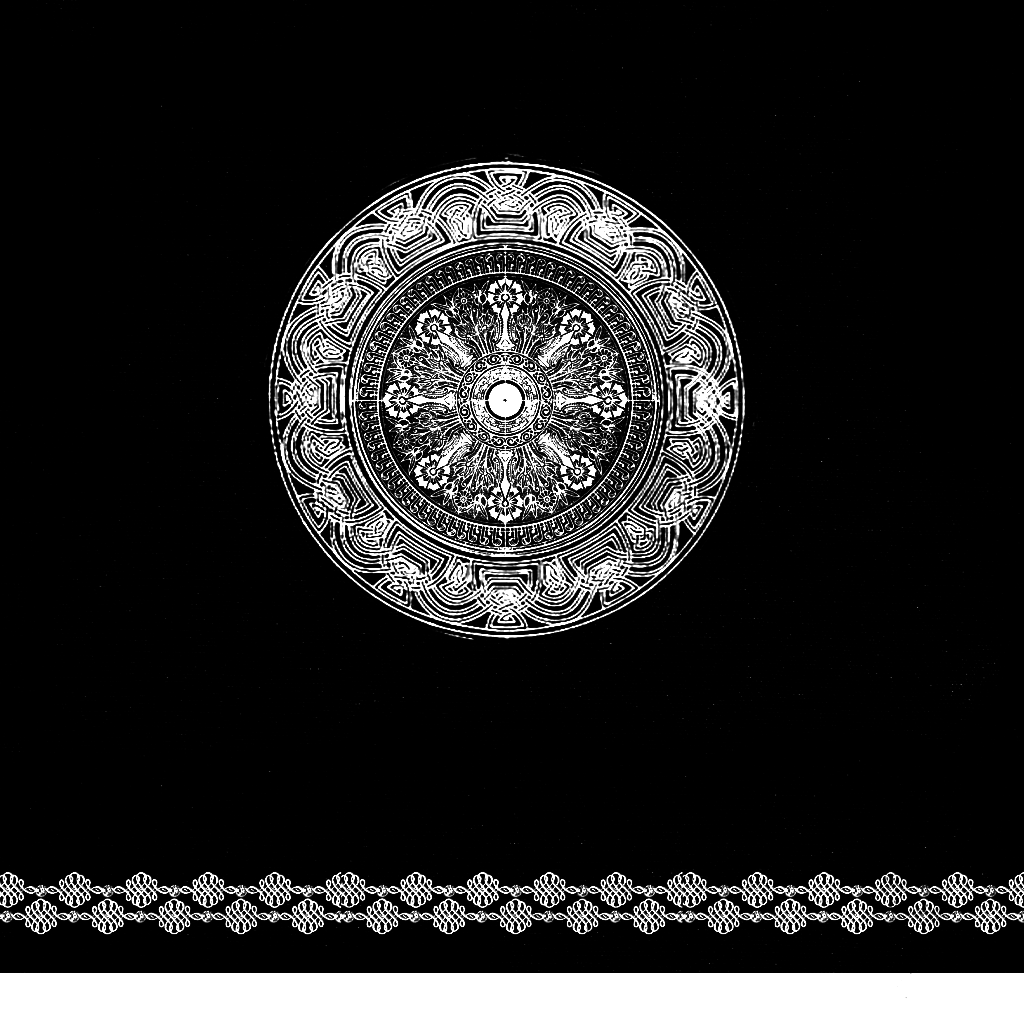
\includegraphics[width=\textwidth]{texture_sample/curtain_metallic}
\end{subfigure} }
\caption{Texture setup demonstrated on curtain from sponza scene.}
\label{fig:texturesample}
\end{figure}
\todo{Move section to the appendix?}
Our material setup resembles what is usually called "metallic setup" in physically based shading (see \autoref{fig:texturesample}).
To parameterize the Blinn Phong BRDF, all surfaces have a reflectance texture (sRGB), tangent space normal-maps and two material property textures which are combined into a single texture during loading if not already in the desired format.
The first channel contains a roughness value $r$ from which we derive the Blinn-Phong specular exponent $\gamma$ and the second determines how metallic a surface is:
Using this metallic value $m$, the reflectance $c$ is split up into diffuse $\rho_d$ and specular reflectance $\rho_s$.
The interpretation of all these values happens at runtime using simple heuristics:
\begin{align}
\gamma &= \frac{2}{r^4 + 0.0005}\\
\rho_d &= c \cdot (1-m) + 0.02 \cdot m\\
\rho_s &= 0.04 \cdot (1-m) + c \cdot m
\end{align}
The exponent computation as well as the base diffuse reflectivity for metallic objects are based on cosmetic considerations.
A specular reflectivity of 0.04 is the average for most dielectrics \cite{bib:natypbr}.

Direct lighting is achieved using a deferred renderer with a floating point depth buffer and three layers:
A sRGB texture containing reflectance, a two channel 16\,bit signed integer layer for angle representation of the normal vector and a 8bit two channel texture for the aforementioned roughness and metallic values.

\subsection{RSM Format}
Like our G-Buffer, the RSM consists of three textures and a floating point depth texture.
As before we store normals compressed by storing their two angles in signed 16 bit integer textures.
We tried to use the low precision floating point format \emph{R11G11B10F} for storing the flux.
This however led to severe artifacts if the RSM is downsampled from a texture which is more than three times larger.
Instead, a three channel 16bit float format is used.
Since we need to downsample depth and squared depth, we added a separate 2 channel 16bit float texture for this purpose.
The full float depth texture is only used as depth buffer during rendering and for direct lighting.

\subsection{Cache Allocation} \label{sec:impl:cachealloc}
For simpler addressability all CAV cascades are stored in the same 32bit integer volume texture.
Since each cascade is cubic and has the same resolution, they can be simply aligned along the x-coordinate.

The task of the cache allocation pass is to find unique addresses for all needed caches and write them into the CAV.
For this, a compute shader with a thread for each screen pixel is dispatched.
Each pixel is only allowed to increase the global cache counter if its destination CAV cell has not already been written.
This can be easily achieved using the compare and swap atomic operation on the CAV cell and an atomic-add on the global cache counter.
The following simplified GLSL code describes how this process works:
\begin{lstlisting}[language=GLSL]
void AllocateCache(uint cascade, uvec3 cachePosition)
{
	uvec3 CAVcoord = cachePosition;
	CAVcoord.x += cascade * AddressVolumeResolution;

	// Try lock.
	uint oldAddressValue = imageAtomicCompSwap(VoxelAddressVolume, CAVcoord, 
                                                uint(0), uint(0xFFFFFFFF));
	// Continue if lock was successful.
	if(oldAddressValue == 0)
	{
		// Increment total cache count and retrieve buffer address.
		uint lightCacheIndex = atomicAdd(TotalLightCacheCount, 1);

		// Compute cache world position and save in global cache buffer.
		LightCacheBuffer[lightCacheIndex].Position = cachePosition *
		                                   AddressVolumeCascades[cascade].WorldVoxelSize +
		                                   AddressVolumeCascades[cascade].Min;

		// Store address. No need for atomic now, since the cell is kept locked.
		// Light cache index 0 is reserved for "empty".
		imageStore(VoxelAddressVolume, unpackedAddressCoord, lightCacheIndex + 1);
	}
}
\end{lstlisting}
Note that this is a very expensive operation (due to the atomics on global memory) which usually executed redundantly since neighboring pixels mark the same caches most of the time.
To reduce the number of such function calls we first tried to implement a cache in shared memory.
However, it turned out the newly introduced atomic operations on shared memory to implement such a cache were even more expensive which limited the efficiency considerably.
\\
Our final version works with shared memory and a simple heuristic that does not rely on atomic operations:
\begin{lstlisting}[language=GLSL]
shared uint cacheList[THREAD_GROUP_SIZE][THREAD_GROUP_SIZE];

// ...

// Retrieve integer that represents the cache coordinate and save it to the shared memory.
int ownCacheCoord = GetCache1DCoord(pixelWorldPosition, addressVolumeCascade);
cacheList[gl_LocalInvocationID.x][gl_LocalInvocationID.y] = ownCacheCoord;

// Wait for all other threads in this group.
barrier();

// Allocate only if there is no thread with a lower number index on any axis
// with the same cache coordinate.
uvec2 lookUpThread = max(uvec2(0), uvec2(gl_LocalInvocationID.xy) - uvec2(1));
if((cacheList[gl_LocalInvocationID.x][lookUpThread.y] != ownCacheCoord && 
    cacheList[lookUpThread.x][gl_LocalInvocationID.y] != ownCacheCoord &&
    cacheList[lookUpThread.x][lookUpThread.y] != ownCacheCoord) ||
   lookUpThread == gl_LocalInvocationID.xy))
{
	// Unpack cache coord and allocate the nearest 8 caches.
	AllocateCaches(ownCacheCoord);
}
\end{lstlisting}
Again, the code was simplified for better readability.
First, every thread writes the packed coordinate of one of its destination caches into shared memory.
Remember that there are actually eight that influence a single pixel.
To simplify the process we consider only the one with the lowest coordinate on all axes.
After a barrier-sync we check if none of the threads to the left, bottom or left-bottom wrote the same coordinate to the cache list.
The most bottom left thread always calls the allocate function - otherwise no cache would be allocated at all if all threads of a group wrote the same cache address.
\\
To handle transitions, we use a second cache list in memory where we apply the same scheme.
As an additional optimization, threads perform the lookup in the opposite direction (top/right), so that it is unlikely that the same thread needs to allocate both the "normal" and the "transition-zone" cache.
\\
We achieved the best performance at with a thread group size of $16\times16$.

For a resolution of $2560\times1440$ and a view with about 16 k caches, our methods is roughly six times faster than the primitive approach.

\subsection{Voxelization \& Shadow Cones}
We use the GPU voxelization as presented by Crassin and Green \cite{bib:openglinsightsvoxel}.
This allows us to recompute the voxelization every frame for a relatively low cost.
Since we save only a 8bit occupancy value, our overall memory consumption stays low.

In order to avoid temporal incoherence that arises when objects are moving through the coarse binary voxelization, we add the difference between the current voxelization to the last one gradually.
Depending on the (manually set) adaption rate, very fast objects may leave only faint traces in the voxel-grid.
In consequence they will cast no or only dim shadows.
The perceptually best adaption rate depends on the relative voxel cell size.
Coarser volumes need slower adaptions since otherwise large shadow features might pop in.

All shadow cones start with an offset which is as large as two voxel cells to reduce the likelihood of accidental self-shadowing. 

\subsection{Cache Lighting} \label{sec:impl:details:lighting}
\begin{figure}[h]
\centering
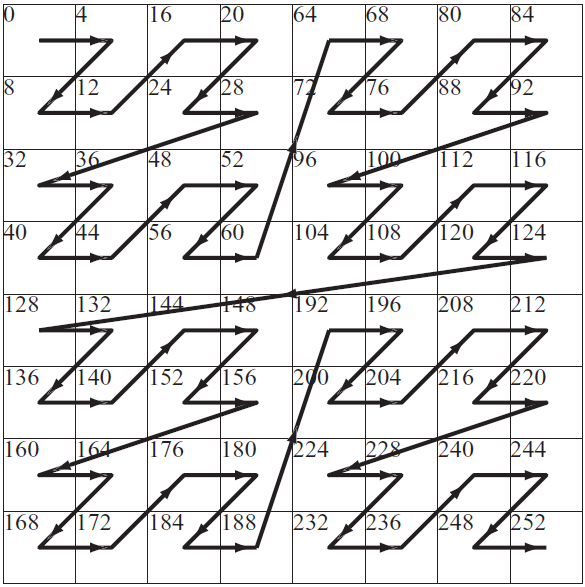
\includegraphics[width=0.5\textwidth]{morton_rtr}
\caption{\cite[p.848]{bib:RealtimeRenderingBook} The Morton sequence pattern. } \label{fig:morton}
\end{figure}
Our shadow LOD algorithm requires that a shadowing value is valid for multiple neighboring virtual lights.
This means that all VALs that share the same shadowing need to be bulk-processed.
To achieve this without having to re-implement the iteration on the RSM for every shadow lod, we use the \emph{Morton sequence} \cite{bib:mortonorder} which is visualized in \autoref{fig:morton}.
Computing the two-dimensional coordinate from a running integer involves several costly integer operations.
However, in some cases the lighting process even speed up in our implementation, most likely since the texture resides in the video ram in exactly this or a similar order \cite[p.848]{bib:RealtimeRenderingBook}.
Note that this more or less forces us to use quadric power of two RSMs since other sizes are more difficult to traverse and introduce exceptions to our shadow sampling scheme.

Since all shader invocations need to load all virtual lights from the RSM, we can easily optimize the texture accesses by first storing lights in the shared memory.
In our tests uncompressing the data (decoding normals, computing position from depth etc.) proved to be beneficial although this takes more shared memory.
The following code fragment illustrates the process:
\begin{lstlisting}[language=GLSL]
shared LightInfo RSMCache[THREADS_PER_GROUP];

// ...

for(uint rsmIndex = gl_LocalInvocationID.x; rsmIndex < totalNumRSMPixels; rsmIndex += THREADS_PER_GROUP)
{
	// Each thread loads a reflective shadow map texel = VAL.
	LightInfo cacheEntry;

	// Unpack rsmIndex to a actual position.
	ivec2 rsmSamplePos = ivec2(Morton_2D_Decode_16bit(rsmIndex)); 

	// Sample flux.
	cacheEntry.Flux = texelFetch(RSM_Flux, rsmSamplePos).rgb;
	// Sample depth and compute VAL area.
	float sourceLightToVAL = texelFetch(RSM_DepthLinSq, rsmSamplePos).r;
	cacheEntry.DiscArea = sourceLightToVAL * sourceLightToVAL * ValAreaFactor;
	// Compute world position.
	cacheEntry.Position = ComputeVALPosition(rsmSamplePos, sourceLightToVAL);
	// Sample and unpack normal.
	cacheEntry.Normal = UnpackNormal16I(texelFetch(RSM_Normal, rsmSamplePos).xy);

	// Write into cache.
	barrier(); // Wait for other threads to load lights.
 	RSMCache[gl_LocalInvocationID.x] = cacheEntry;
	barrier(); // Make sure all other threads have written their lights.

	// Perform lighting for all cached lights.
	float visibility = 1.0;
	for(int i=0; i<LIGHTING_THREADS_PER_GROUP; ++i)
	{
		if(i % IndirectShadowComputationSampleInterval == 0)
		{
			shadowing = ComputeConeTraceShadow(/* ... */);
		}
		
		PerformLighting(RSMCache[i].Flux, visibility, /* ... */);
	}
}

// Write lighting results to cache buffer.
// ...
\end{lstlisting}
Each compute shader thread of a group loads exactly one light into the shared memory, waits for all other threads of its group and then starts to traverse the lights cached in the shared memory.
This is repeat until all virtual lights have been processed.

\subsubsection{Specular Lighting} \label{sec:impl:details:specular}
For the specular environment map atlas we use the low precision floating point format \emph{R11G11B10F}.
\\
There are two different ways to handle writes to this texture.
One way is simply to write values in just the moment they are computed.
However, since multiple VALs might address the same pixel in the specular environment map, a read has to be performed first to add the radiance instead of overwriting existing information.
Because of this we experimented with a cached write:
Each thread holds its portion of the texture first in its registers.
Since even for low resolutions this creates a very high register pressure, it is cheaper to compress this in-memory map.
As it is expensive to de-/compress from/to \emph{R11G11B10F} in software, we use a custom 32 bit shared exponent format for this task.
\\
Due to the different highly lossy compressions both methods yield visually different results.
\autoref{sec:eva:specperf} discusses which technique performs better.


\subfilebib % Makes bibliography available when compiling as subfile
\end{document}